% SPDX-License-Identifier: CC-BY-SA-4.0
% Author: Matthieu Perrin
% Part: 
% Section: 
% Sub-section: 
% Frame: 

\begingroup

\begin{frame}[fragile]{Un algorithme de liste chaînée}

  \vspace{15mm}
  \begin{lstlisting}[gobble=4]
    public class Queue<T> {
      private class Node {
        (*\Example<2>{T value;}*)
        (*\Alert<2>{Node next = null;}*)
        Node(T val) { (*\Example<2>{value = val;}*) }
      }
      
      private (*\Alert<2>{Node first = new Node(null);}*)
      private (*\Alert<2>{Node last = head;}*)

      public void (*\Structure<1>{enqueue(T value)}*) {
        last.(*\Alert<2>{next}*) = new Node(value);
        (*\Alert<2>{last}*) = last.next;
      }
      
      public T (*\Structure<1>{dequeue()}*) {
        if(first == last) return null;
        (*\Alert<2>{first}*) = first.next;
        return first.value;
      }
    }
  \end{lstlisting}

  \on[y=25mm]{
    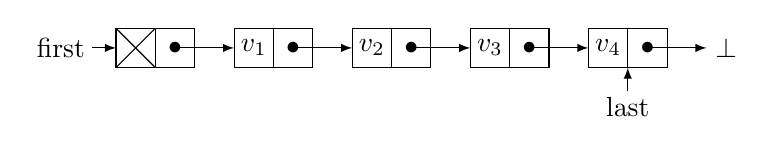
\begin{tikzpicture}
      \draw (-.7,.25) node{first};
      \draw (6.5,-.5) node{last};
      
      \draw[-latex] (-.3,0.25) -- (0,0.25);
      \draw[-latex] (6.5,-.3) -- (6.5,0);

      \draw (0.0,0) rectangle +(.5,.5) rectangle +(1,0) +(.75,.25) node{$\bullet$};
      \draw (1.5,0) rectangle +(.5,.5) rectangle +(1,0) +(.25,.25) node{$v_1$}  +(.75,.25) node{$\bullet$};
      \draw (3.0,0) rectangle +(.5,.5) rectangle +(1,0) +(.25,.25) node{$v_2$}  +(.75,.25) node{$\bullet$};
      \draw (4.5,0) rectangle +(.5,.5) rectangle +(1,0) +(.25,.25) node{$v_3$}  +(.75,.25) node{$\bullet$};
      \draw (6.0,0) rectangle +(.5,.5) rectangle +(1,0) +(.25,.25) node{$v_4$}  +(.75,.25) node{$\bullet$};
      \draw[-latex] (0.0,0) +(.75,.25) -- +(1.5,.25);
      \draw[-latex] (1.5,0) +(.75,.25) -- +(1.5,.25);
      \draw[-latex] (3.0,0) +(.75,.25) -- +(1.5,.25);
      \draw[-latex] (4.5,0) +(.75,.25) -- +(1.5,.25);
      \draw[-latex] (6.0,0) +(.75,.25) -- +(1.5,.25);
      \draw (7.5,0) +(.25,.25) node{$\bot$} ;

      \draw (0,0) -- (.5,.5);
      \draw (0,.5) -- (.5,0);
    \end{tikzpicture}
  }
  
  \onBlock[right=40mm, y=5mm]{File vide}{
    \centering
    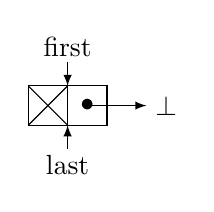
\begin{tikzpicture}
      \draw (6.5,-2) node{first};
      \draw (6.5,-3.5) node{last};
      
      \draw[-latex] (6.5,-2.2) -- (6.5,-2.5);
      \draw[-latex] (6.5,-3.3) -- (6.5,-3);

      \draw (6,-3) rectangle +(.5,.5) rectangle +(1,0) +(.75,.25) node{$\bullet$};
      \draw[-latex] (6,-3) +(.75,.25) -- +(1.5,.25);
      \draw (7.5,-3) +(.25,.25) node{$\bot$} ;
      \draw (6,-3) -- (6.5,-2.5);
      \draw (6,-2.5) -- (6.5,-3);
    \end{tikzpicture}
  }

  \onBlock[right=40mm, y=-25mm]{Conseils}{
    \begin{enumerate}
    \item Écrire le code séquentiel
    \item<2> identifier les variables
      \begin{itemize}
      \item {\color{exampleColor}constantes}
      \item \alert{mutables}
      \end{itemize}
    \end{enumerate}
  }
  
\end{frame}

\endgroup
\endinput
